
\section{Interpretation of Results}
\label{sec:interpretation_of_results}
The quantitative and qualitative analyses together provide a comprehensive understanding of the strengths and limitations of our weakly supervised segmentation framework.

From the quantitative perspective, the model achieves a mean IoU of 50.3\% on the validation set and 50.8\% on the test set, indicating strong generalization despite using only weak supervision. The per-class IoU breakdown (Table~\ref{tab:per_class_iou_comparison}) reveals that large and distinctive object categories—such as \textbf{bus}, \textbf{sheep}, \textbf{horse}, and \textbf{cat}—are segmented with high accuracy, while classes that are small, highly deformable, or poorly represented during pretraining (e.g., \textbf{person}, \textbf{chair}, and \textbf{potted plant}) show significantly weaker performance. This pattern aligns with the biases inherent in the pretraining datasets (ImageNet-21K and YFCC-14M), which lack dense, diverse coverage for these semantic categories.

Qualitative inspection further supports these findings. Visual examples show that predictions for animals and vehicles tend to produce coherent and complete masks with clear object boundaries, whereas human instances often exhibit fragmented or overly diffuse activations. In particular, the \textbf{person} class consistently fails due to its initial Class Activation Maps (CAMs) being dominated by high confidence in the \textbf{background} regions. Since the Refinement Module (RFM) operates via random walk propagation, these early misaligned activations are spread across spatially adjacent pixels, reinforcing incorrect background predictions. Moreover, the pixel-adaptive module, while effective in smoothing object interiors, tends to over-suppress fine structural details in thin or articulated objects such as limbs, further degrading segmentation quality for humans.

Overall, the results indicate that our model is highly effective in identifying large, contextually distinct objects but remains sensitive to CAM initialization errors and class imbalance during pretraining. The analysis suggests that improving CAM reliability—particularly for human-centric and small-object categories—through better initialization, adaptive refinement control, or scale-aware feature fusion could significantly enhance overall segmentation quality.

\begin{figure}[H]
  \centering
  \setlength{\tabcolsep}{2pt} % adjust spacing
  \renewcommand{\arraystretch}{0.9}
  % Wrap the table in a colored box (requires \usepackage{tcolorbox})
  \begin{tcolorbox}[colframe=black!60, colback=white, boxrule=0.8pt, arc=2pt, left=2pt, right=2pt, top=2pt, bottom=2pt]
    \centering
    \begin{tabular}{cccc}
      (a) Input & (b) GT & (c) WeCLIP & (d) Ours           \\
      [1mm]

      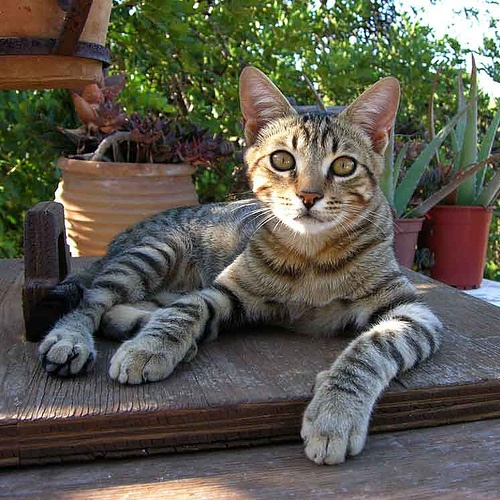
\includegraphics[width=0.20\textwidth,height=0.20\textwidth]
      {figures/originals/2007_003778}
                &
      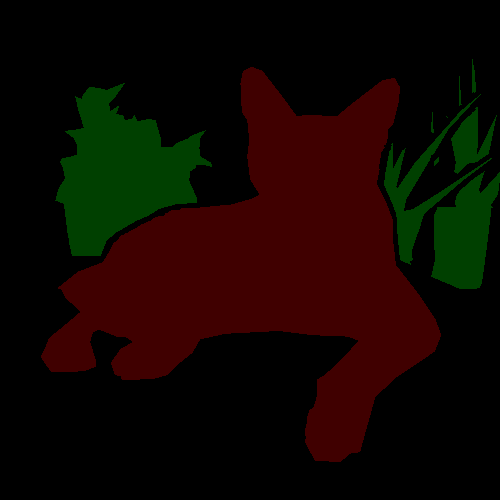
\includegraphics[width=0.20\textwidth,height=0.20\textwidth]
      {figures/colored_gts/2007_003778}
                &
      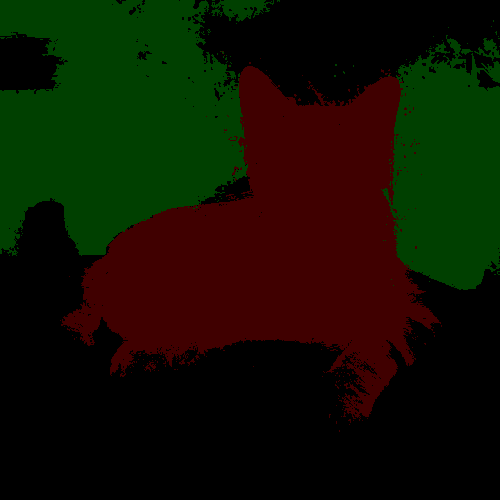
\includegraphics[width=0.20\textwidth,height=0.20\textwidth]
      {figures/val_labels/weclip/2007_003778_[7, 15]}
                &
      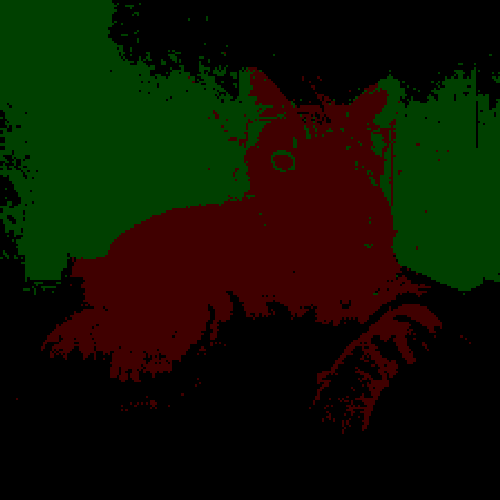
\includegraphics[width=0.20\textwidth,height=0.20\textwidth]
      {figures/val_labels/ours/2007_003778_[7, 15]}    \\

      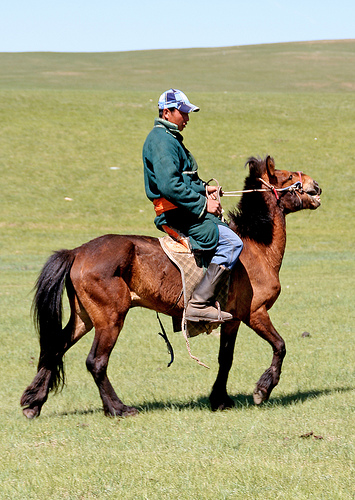
\includegraphics[width=0.20\textwidth,height=0.20\textwidth]
      {figures/originals/2009_003768}
                &
      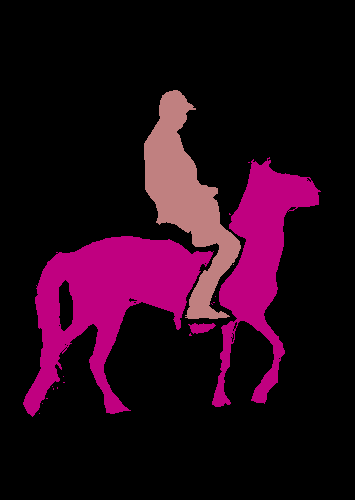
\includegraphics[width=0.20\textwidth,height=0.20\textwidth]
      {figures/colored_gts/2009_003768}
                &
      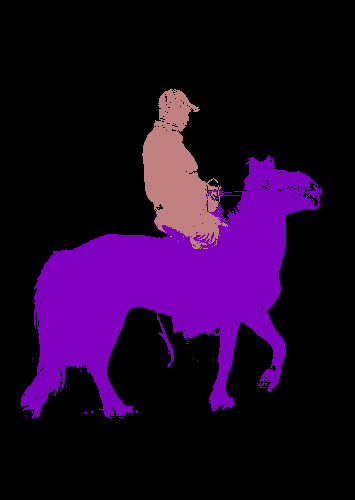
\includegraphics[width=0.20\textwidth,height=0.20\textwidth]
      {figures/val_labels/weclip/2009_003768_[12, 14]}
                &
      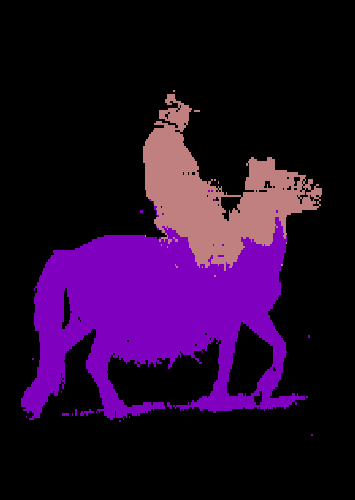
\includegraphics[width=0.20\textwidth,height=0.20\textwidth]
      {figures/val_labels/ours/2009_003768_[12, 14]}   \\

      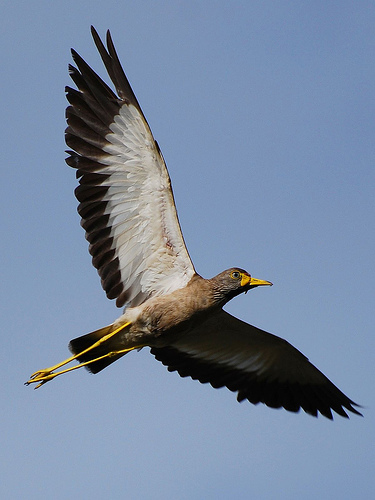
\includegraphics[width=0.20\textwidth,height=0.20\textwidth]
      {figures/originals/2011_001967}
                &
      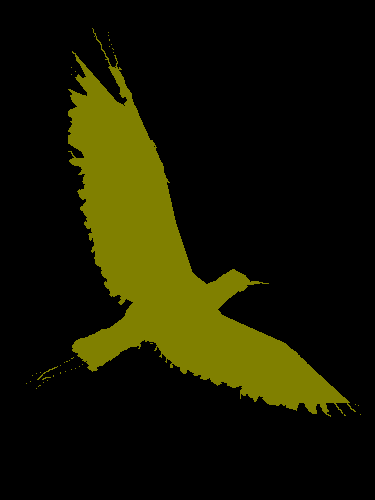
\includegraphics[width=0.20\textwidth,height=0.20\textwidth]
      {figures/colored_gts/2011_001967}
                &
      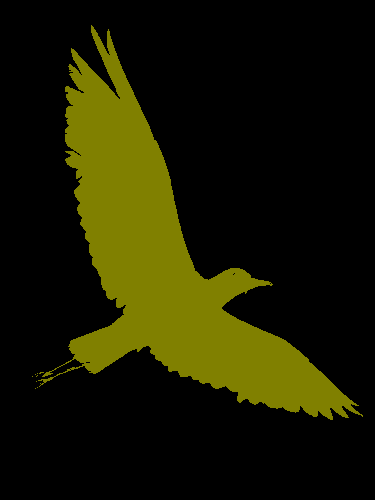
\includegraphics[width=0.20\textwidth,height=0.20\textwidth]
      {figures/val_labels/weclip/2011_001967_[2]}
                &
      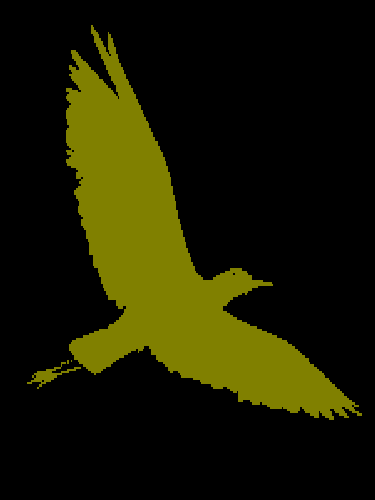
\includegraphics[width=0.20\textwidth,height=0.20\textwidth]
      {figures/val_labels/ours/2011_001967_[2]}        \\


      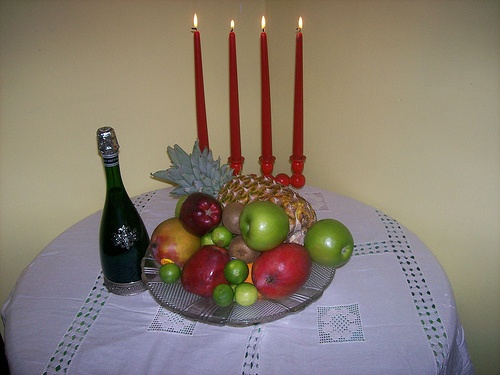
\includegraphics[width=0.20\textwidth,height=0.20\textwidth]
      {figures/originals/2007_000250}
                &
      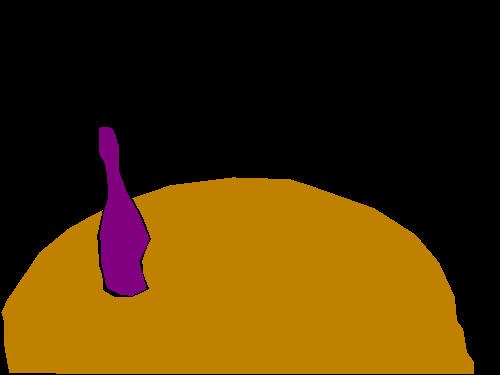
\includegraphics[width=0.20\textwidth,height=0.20\textwidth]
      {figures/colored_gts/2007_000250}
                &
      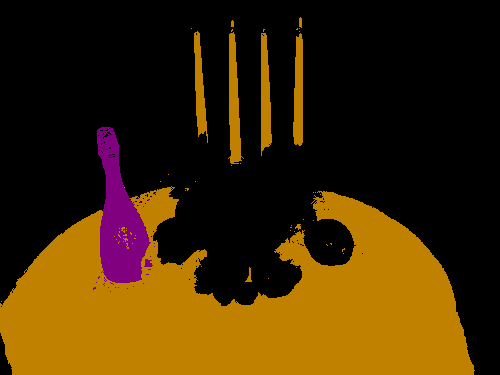
\includegraphics[width=0.20\textwidth,height=0.20\textwidth]
      {figures/val_labels/weclip/2007_000250_[4, 10]}
                &
      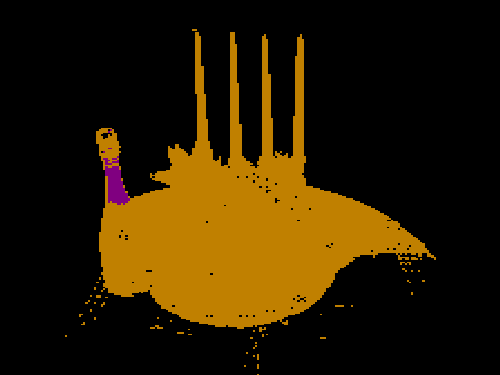
\includegraphics[width=0.20\textwidth,height=0.20\textwidth]
      {figures/val_labels/ours/2007_000250_[4, 10]}    \\


      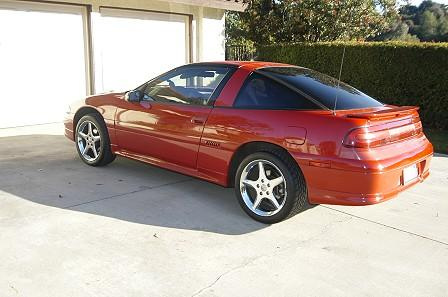
\includegraphics[width=0.20\textwidth,height=0.20\textwidth]
      {figures/originals/2010_005119}
                &
      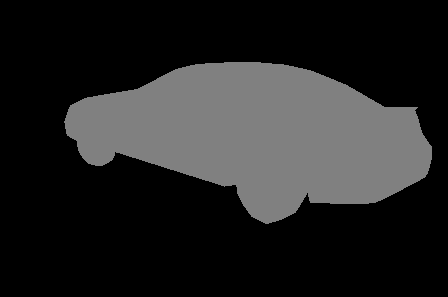
\includegraphics[width=0.20\textwidth,height=0.20\textwidth]
      {figures/colored_gts/2010_005119}
                &
      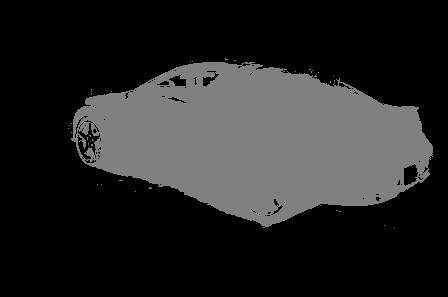
\includegraphics[width=0.20\textwidth,height=0.20\textwidth]
      {figures/val_labels/weclip/2010_005119_[6]}
                &
      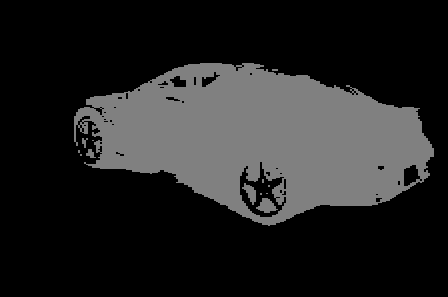
\includegraphics[width=0.20\textwidth,height=0.20\textwidth]
      {figures/val_labels/ours/2010_005119_[6]}        \\



      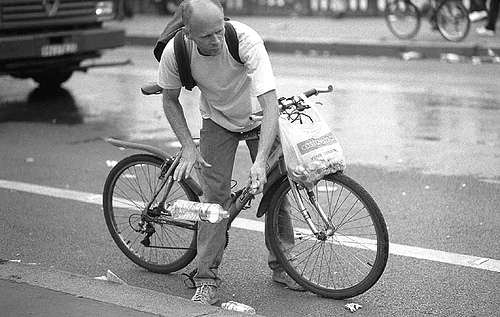
\includegraphics[width=0.20\textwidth,height=0.20\textwidth]
      {figures/originals/2011_000453}
                &
      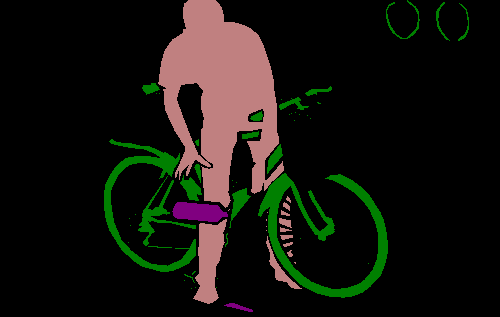
\includegraphics[width=0.20\textwidth,height=0.20\textwidth]
      {figures/colored_gts/2011_000453}
                &
      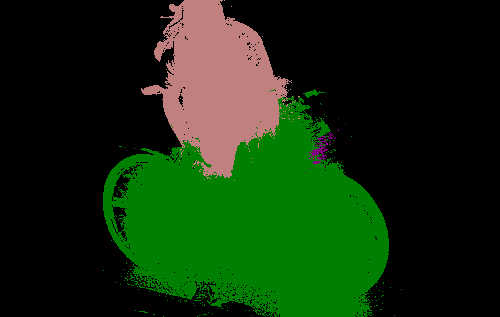
\includegraphics[width=0.20\textwidth,height=0.20\textwidth]
      {figures/val_labels/weclip/2011_000453_[1, 4, 14]}
                &
      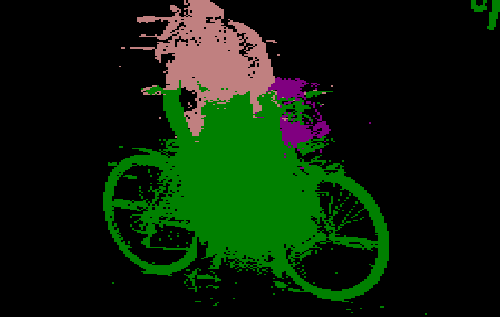
\includegraphics[width=0.20\textwidth,height=0.20\textwidth]
      {figures/val_labels/ours/2011_000453_[1, 4, 14]} \\

      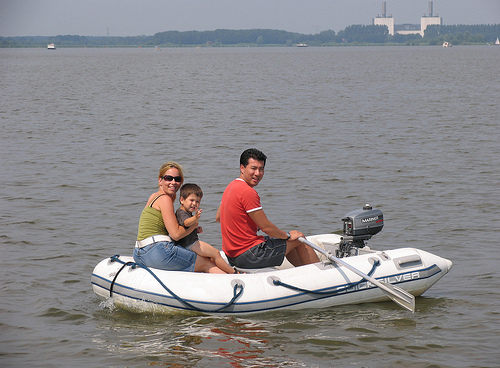
\includegraphics[width=0.20\textwidth,height=0.20\textwidth]
      {figures/originals/2010_003599}
                &
      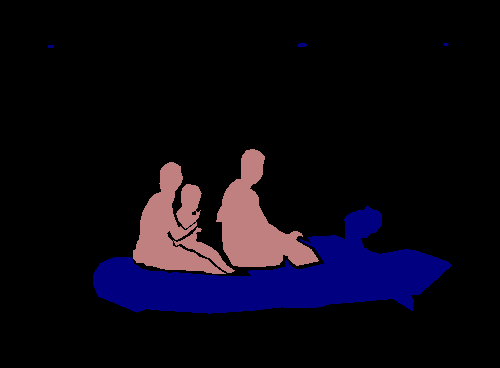
\includegraphics[width=0.20\textwidth,height=0.20\textwidth]
      {figures/colored_gts/2010_003599}
                &
      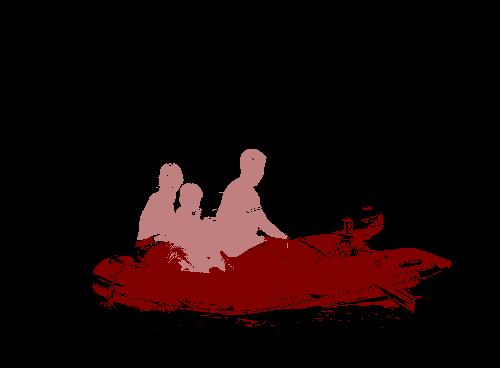
\includegraphics[width=0.20\textwidth,height=0.20\textwidth]
      {figures/val_labels/weclip/2010_003599_[3, 14]}
                &
      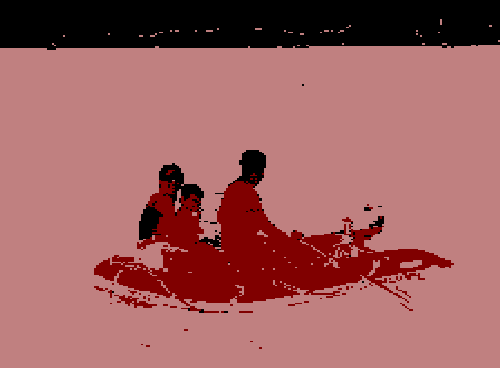
\includegraphics[width=0.20\textwidth,height=0.20\textwidth]
      {figures/val_labels/ours/2010_003599_[3, 14]} \\
    \end{tabular}

    \caption{Qualitative comparison of pseudo-labels between WeCLIP and our UniCL-AffSeg on PASCAL VOC 2012 \textit{val} set.}
    \label{fig:qualitative_comparison_pseudolabel_val}
  \end{tcolorbox}
\end{figure}


\begin{figure}[H]
  \centering
  \setlength{\tabcolsep}{2pt} % adjust spacing
  \renewcommand{\arraystretch}{0.9}
  % Wrap the table in a colored box (requires \usepackage{tcolorbox})
  \begin{tcolorbox}[colframe=black!60, colback=white, boxrule=0.8pt, arc=2pt, left=2pt, right=2pt, top=2pt, bottom=2pt]
    \centering
    \begin{tabular}{cccc}
      (a) Input & (b) GT & (c) WeCLIP & (d) (Ours)           \\
      [1mm]

      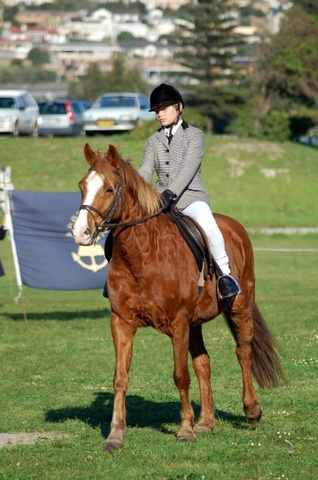
\includegraphics[width=0.20\textwidth,height=0.20\textwidth]
      {figures/originals/2007_005331}
                &
      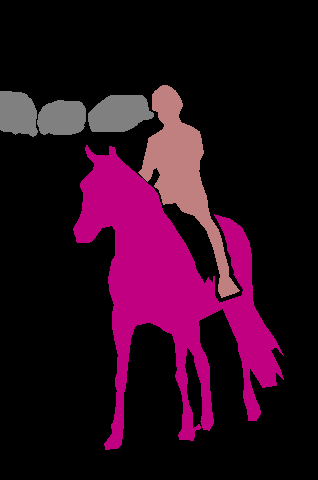
\includegraphics[width=0.20\textwidth,height=0.20\textwidth]
      {figures/colored_gts/2007_005331}
                &
      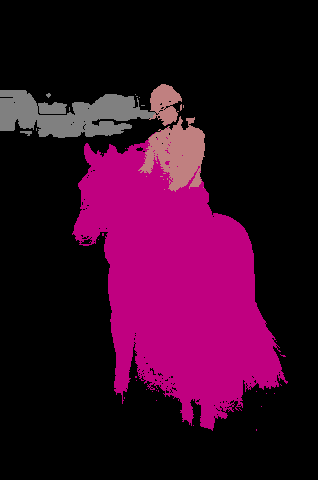
\includegraphics[width=0.20\textwidth,height=0.20\textwidth]
      {figures/test_labels/weclip/2007_005331_[6, 12, 14]}
                &
      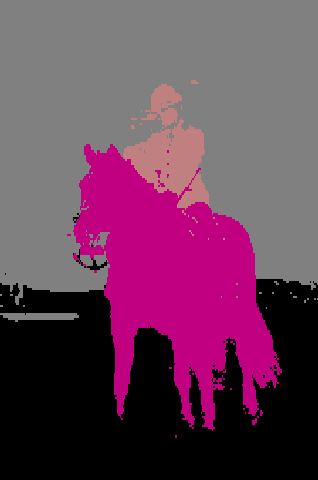
\includegraphics[width=0.20\textwidth,height=0.20\textwidth]
      {figures/test_labels/ours/2007_005331_[6, 12, 14]}    \\

      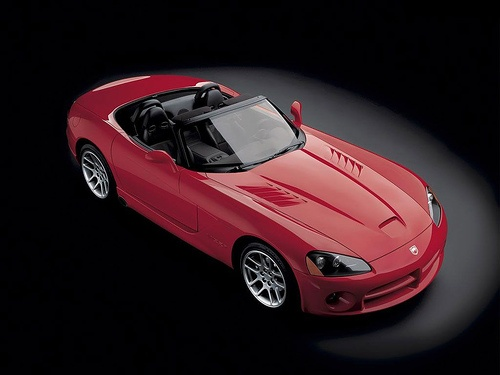
\includegraphics[width=0.20\textwidth,height=0.20\textwidth]
      {figures/originals/2007_006277}
                &
      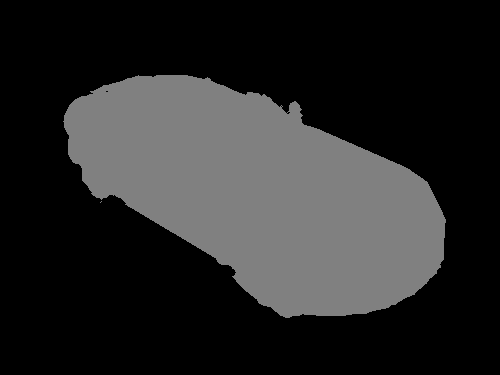
\includegraphics[width=0.20\textwidth,height=0.20\textwidth]
      {figures/colored_gts/2007_006277}
                &
      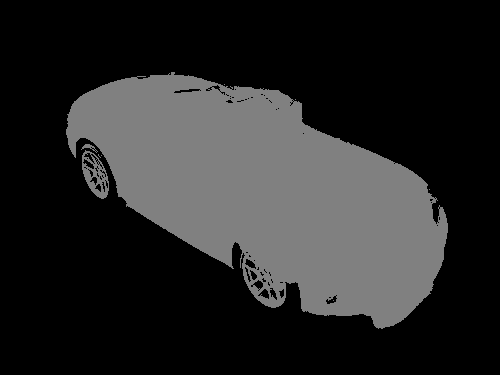
\includegraphics[width=0.20\textwidth,height=0.20\textwidth]
      {figures/test_labels/weclip/2007_006277_[6]}
                &
      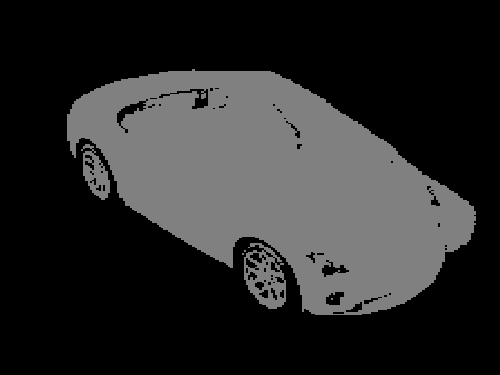
\includegraphics[width=0.20\textwidth,height=0.20\textwidth]
      {figures/test_labels/ours/2007_006277_[6]}   \\

      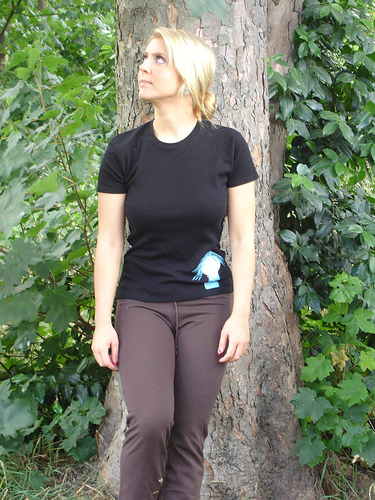
\includegraphics[width=0.20\textwidth,height=0.20\textwidth]
      {figures/originals/2008_001504}
                &
      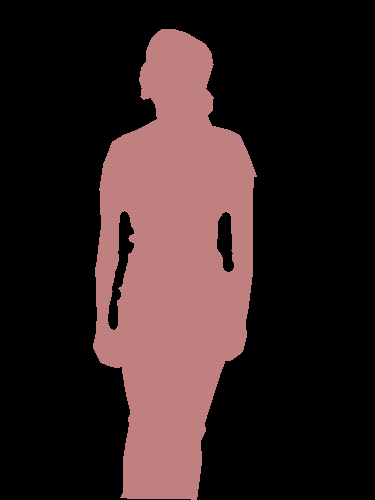
\includegraphics[width=0.20\textwidth,height=0.20\textwidth]
      {figures/colored_gts/2008_001504}
                &
      \includegraphics[width=0.20\textwidth,height=0.20\textwidth]
      {figures/test_labels/weclip/2008_001504_[14]}
                &
      \includegraphics[width=0.20\textwidth,height=0.20\textwidth]
      {{figures/test_labels/ours/2008_001504_[14]}}        \\


      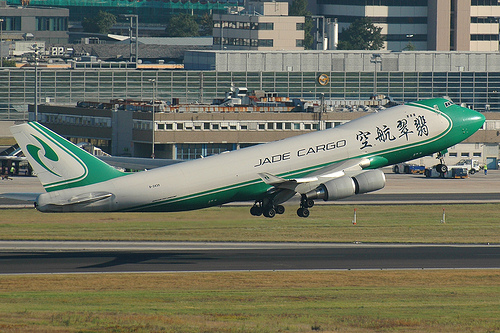
\includegraphics[width=0.20\textwidth,height=0.20\textwidth]
            {figures/originals/2008_002358}
                &
      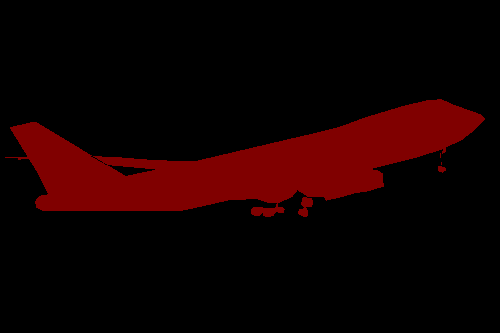
\includegraphics[width=0.20\textwidth,height=0.20\textwidth]
      {figures/colored_gts/2008_002358}
                &
      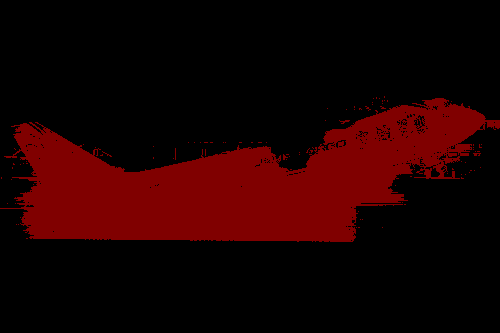
\includegraphics[width=0.20\textwidth,height=0.20\textwidth]
      {figures/test_labels/weclip/2008_002358_[0]}
                &
      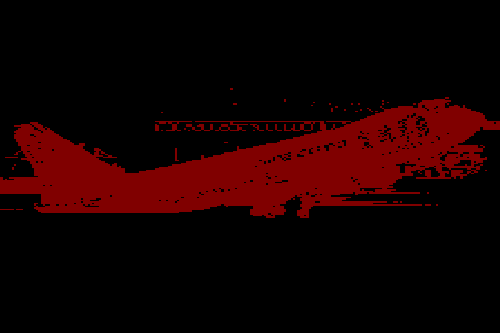
\includegraphics[width=0.20\textwidth,height=0.20\textwidth]
      {figures/test_labels/ours/2008_002358_[0]}    \\


      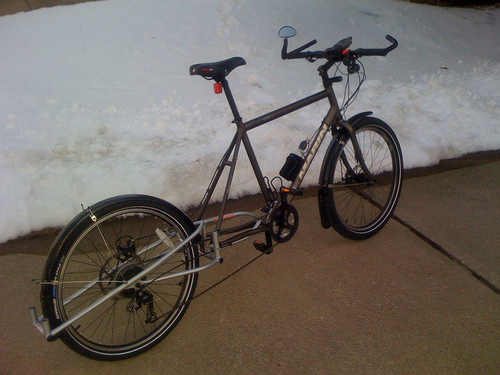
\includegraphics[width=0.20\textwidth,height=0.20\textwidth]
      {figures/originals/2009_003224}
                &
      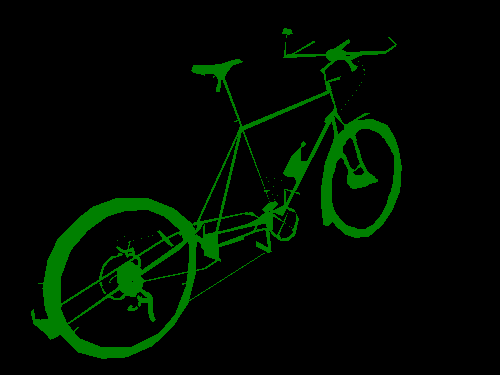
\includegraphics[width=0.20\textwidth,height=0.20\textwidth]
      {figures/colored_gts/2009_003224}
                &
      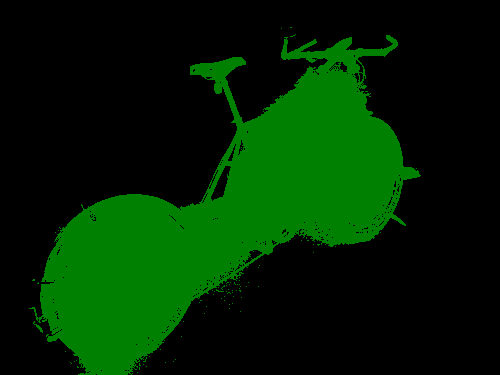
\includegraphics[width=0.20\textwidth,height=0.20\textwidth]
      {figures/test_labels/weclip/2009_003224_[1]}
                &
      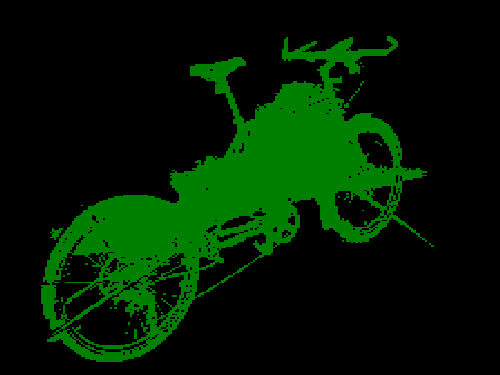
\includegraphics[width=0.20\textwidth,height=0.20\textwidth]
      {figures/test_labels/ours/2009_003224_[1]}        \\



      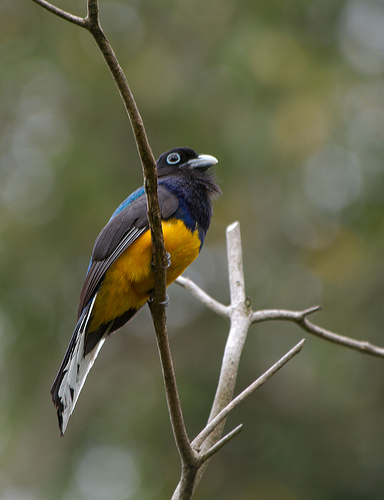
\includegraphics[width=0.20\textwidth,height=0.20\textwidth]
      {figures/originals/2009_004084}
                &
      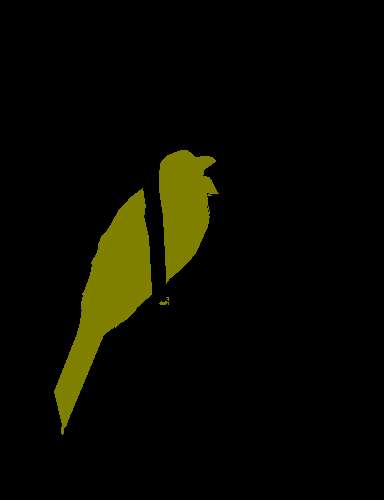
\includegraphics[width=0.20\textwidth,height=0.20\textwidth]
      {figures/colored_gts/2009_004084}
                &
      \includegraphics[width=0.20\textwidth,height=0.20\textwidth]
      {figures/test_labels/weclip/2009_004084_[2]}
                &
      \includegraphics[width=0.20\textwidth,height=0.20\textwidth]
      {figures/test_labels/ours/2009_004084_[2]} \\

      
      \includegraphics[width=0.20\textwidth,height=0.20\textwidth]
      {figures/originals/2010_002531}
                &
      \includegraphics[width=0.20\textwidth,height=0.20\textwidth]
      {figures/colored_gts/2010_002531}
                &
      \includegraphics[width=0.20\textwidth,height=0.20\textwidth]
      {figures/test_labels/weclip/2010_002531_[7, 17]}
                &
      \includegraphics[width=0.20\textwidth,height=0.20\textwidth]
      {figures/test_labels/ours/2010_002531_[7, 17]} \\


    \end{tabular}

    \caption{Qualitative comparison of pseudo-labels between WeCLIP and our UniCL-AffSeg on PASCAL VOC 2012 \textit{test} set.}
    \label{fig:qualitative_comparison_pseudolabel_test}
  \end{tcolorbox}
\end{figure}



\begin{figure}[H]
  \centering
  \setlength{\tabcolsep}{2pt} % adjust spacing
  \renewcommand{\arraystretch}{0.9}
  % Wrap the table in a colored box (requires \usepackage{tcolorbox})
  \begin{tcolorbox}[colframe=black!60, colback=white, boxrule=0.8pt, arc=2pt, left=2pt, right=2pt, top=2pt, bottom=2pt]
    \centering
    \begin{tabular}{cccc}
      (a) Input & (b) GT & (c) WeCLIP & (d) (Ours)           \\
      [1mm]

      \includegraphics[width=0.20\textwidth,height=0.20\textwidth]
      {figures/person_and_chair/originals/2007_000783}
                &
      \includegraphics[width=0.20\textwidth,height=0.20\textwidth]
      {figures/person_and_chair/gt/2007_000783}
                &
      \includegraphics[width=0.20\textwidth,height=0.20\textwidth]
      {figures/person_and_chair/weclip/2007_000783_[12, 14]}
                &
      \includegraphics[width=0.20\textwidth,height=0.20\textwidth]
      {figures/person_and_chair/ours/2007_000783_[12, 14]}    \\

      \includegraphics[width=0.20\textwidth,height=0.20\textwidth]
      {figures/person_and_chair/originals/2007_002824}
                &
      \includegraphics[width=0.20\textwidth,height=0.20\textwidth]
      {figures/person_and_chair/gt/2007_002824}
                &
      \includegraphics[width=0.20\textwidth,height=0.20\textwidth]
      {figures/person_and_chair/weclip/2007_002824_[14]}
                &
      \includegraphics[width=0.20\textwidth,height=0.20\textwidth]
      {figures/person_and_chair/ours/2007_002824_[14]}    \\

      \includegraphics[width=0.20\textwidth,height=0.20\textwidth]
      {figures/person_and_chair/originals/2007_004405}
                &
      \includegraphics[width=0.20\textwidth,height=0.20\textwidth]
      {figures/person_and_chair/gt/2007_004405}
                &
      \includegraphics[width=0.20\textwidth,height=0.20\textwidth]
      {figures/person_and_chair/weclip/2007_004405_[8, 10]}
                &
      \includegraphics[width=0.20\textwidth,height=0.20\textwidth]
      {figures/person_and_chair/ours/2007_004405_[8, 10]}    \\


      \includegraphics[width=0.20\textwidth,height=0.20\textwidth]
      {figures/person_and_chair/originals/2007_005702}
                &
      \includegraphics[width=0.20\textwidth,height=0.20\textwidth]
      {figures/person_and_chair/gt/2007_005702}
                &
      \includegraphics[width=0.20\textwidth,height=0.20\textwidth]
      {figures/person_and_chair/weclip/2007_005702_[1, 14]}
                &
      \includegraphics[width=0.20\textwidth,height=0.20\textwidth]
      {figures/person_and_chair/ours/2007_005702_[1, 14]}    \\


      \includegraphics[width=0.20\textwidth,height=0.20\textwidth]
      {figures/person_and_chair/originals/2011_000713}
                &
      \includegraphics[width=0.20\textwidth,height=0.20\textwidth]
      {figures/person_and_chair/gt/2011_000713}
                &
      \includegraphics[width=0.20\textwidth,height=0.20\textwidth]
      {figures/person_and_chair/weclip/2011_000713_[4, 14]}
                &
      \includegraphics[width=0.20\textwidth,height=0.20\textwidth]
      {figures/person_and_chair/ours/2011_000713_[4, 14]}    \\



      \includegraphics[width=0.20\textwidth,height=0.20\textwidth]
      {figures/person_and_chair/originals/2008_000510}
                &
      \includegraphics[width=0.20\textwidth,height=0.20\textwidth]
      {figures/person_and_chair/gt/2008_000510}
                &
      \includegraphics[width=0.20\textwidth,height=0.20\textwidth]
      {figures/person_and_chair/weclip/2008_000510_[14]}
                &
      \includegraphics[width=0.20\textwidth,height=0.20\textwidth]
      {figures/person_and_chair/ours/2008_000510_[14]}    \\

      
      \includegraphics[width=0.20\textwidth,height=0.20\textwidth]
      {figures/person_and_chair/originals/2008_003477}
                &
      \includegraphics[width=0.20\textwidth,height=0.20\textwidth]
      {figures/person_and_chair/gt/2008_003477}
                &
      \includegraphics[width=0.20\textwidth,height=0.20\textwidth]
      {figures/person_and_chair/weclip/2008_003477_[8, 10]}
                &
      \includegraphics[width=0.20\textwidth,height=0.20\textwidth]
      {figures/person_and_chair/ours/2008_003477_[8, 10]}    \\


    \end{tabular}

    \caption{Qualitative comparison of pseudo-labels between WeCLIP and our UniCL-AffSeg on PASCAL VOC 2012 \textit{val} and \textit{test} set for person and chair classes.}
    \label{fig:qualitative_comparison_pseudolabel_person_chair}
  \end{tcolorbox}
\end{figure}
